%
% Template Laporan Skripsi/Thesis 
%
% @author  Andreas Febrian, Lia Sadita 
% @version 1.03
%
% Dokumen ini dibuat berdasarkan standar IEEE dalam membuat class untuk 
% LaTeX dan konfigurasi LaTeX yang digunakan Fahrurrozi Rahman ketika 
% membuat laporan skripsi. Konfigurasi yang lama telah disesuaikan dengan 
% aturan penulisan thesis yang dikeluarkan UI pada tahun 2008.
%

%
% Tipe dokumen adalah report dengan satu kolom. 
%
\documentclass[12pt, a4paper, onecolumn, oneside, final]{report}

% Load konfigurasi LaTeX untuk tipe laporan thesis
\usepackage{uithesis}
\usepackage{natbib}
\usepackage{import}
% Load konfigurasi khusus untuk laporan yang sedang dibuat
%-----------------------------------------------------------------------------%
% Informasi Mengenai Dokumen
%-----------------------------------------------------------------------------%
% 
% Judul laporan. 
\var{\judul}{Judul Sesuatu Banget \f{English} Miring Juga}
% 
% Tulis kembali judul laporan, kali ini akan diubah menjadi huruf kapital
\Var{\Judul}{JUDUL SESUATU BANGET \f{ENGLISH} MIRING JUGA}
% 
% Tulis kembali judul laporan namun dengan bahasa Ingris
\var{\judulInggris}{Sesuatu Banget in English}

% 
% Tipe laporan, dapat berisi Skripsi, Tugas Akhir, Thesis, atau Disertasi
\var{\type}{Tugas Akhir}
% 
% Tulis kembali tipe laporan, kali ini akan diubah menjadi huruf kapital
\Var{\Type}{Tugas Akhir}
% 
% Tulis nama penulis 
\var{\penulis}{Tegar Aldina Galari}
% 
% Tulis kembali nama penulis, kali ini akan diubah menjadi huruf kapital
\Var{\Penulis}{Tegar Aldina Galari}
% 
% Tulis NPM penulis
\var{\npm}{1306407376}
% 
% Tuliskan Fakultas dimana penulis berada
\Var{\Fakultas}{Ilmu Komputer}
\var{\fakultas}{Ilmu Komputer}
% 
% Tuliskan Program Studi yang diambil penulis
\Var{\Program}{Ilmu Komputer}
\var{\program}{Ilmu Komputer }
\var{\programEng}{Computer Science}
% 
% Tuliskan tahun publikasi laporan
\Var{\bulanTahun}{Juli 2017}
% 
% Tuliskan gelar yang akan diperoleh dengan menyerahkan laporan ini
\var{\gelar}{Sarjana Ilmu Komputer}
% 
% Tuliskan tanggal pengesahan laporan, waktu dimana laporan diserahkan ke 
% penguji/sekretariat
\var{\tanggalPengesahan}{21 Juni 2013} 
% 
% Tuliskan tanggal keputusan sidang dikeluarkan dan penulis dinyatakan 
% lulus/tidak lulus
\var{\tanggalLulus}{5 Juli 2013}
% 
% Tuliskan pembimbing 
\var{\pembimbing}{Prof. Saya }
\var{\pembimbingdua}{Dia S.Kom, M.Kom}
%
% Tuliskan tempat anda kuliah
\var{\kampus}{Universitas Indonesia }
% 
% Alias untuk memudahkan alur penulisan paa saat menulis laporan
\var{\Saya}{Penulis }
\var{\saya}{penulis }

%-----------------------------------------------------------------------------%
% Judul Setiap Bab
%-----------------------------------------------------------------------------%
% 
% Berikut ada judul-judul setiap bab. 
% Silahkan diubah sesuai dengan kebutuhan. 
% 
\Var{\kataPengantar}{Kata Pengantar}
\Var{\babSatu}{Pendahuluan}
\Var{\babDua}{Landasan Teori}
\Var{\babTiga}{Metodologi Penelitian}
\Var{\babEmpat}{Perancangan Implementasi dan Analisis}
\Var{\babLima}{Implementasi dan Pengujian}
\Var{\babEnam}{Hasil Implementasi dan Evaluasi}
\Var{\babTujuh}{Kesimpulan dan Saran}

% Berikut singkatan singkatan yang sering digunakan
% Informasi teknologi asosiasi amerika
\var{\ITTA}{Information Technology Assiciation of America }

\var{\kemkominfo}{Kementrian Komunikasi dan Informasi }
\var{\game}{\textit{video game }}
\var{\ddp}{dasar dasar pemograman }
\var{\DDP}{Dasar dasar pemograman }
\var{\topik}{Iterator }
% Daftar pemenggalan suku kata dan istilah dalam LaTeX
%
% Hyphenation untuk Indonesia 
%
% @author  Andreas Febrian
% @version 1.00
% 
% Tambahkan cara pemenggalan kata-kata yang salah dipenggal secara otomatis 
% oleh LaTeX. Jika kata tersebut dapat dipenggal dengan benar, maka tidak 
% perlu ditambahkan dalam berkas ini. Tanda pemenggalan kata menggunakan 
% tanda '-'; contoh:
% menarik
%   --> pemenggalan: me-na-rik
%

\hyphenation{
    % alphabhet A
    a-na-li-sa a-tur 
    a-pli-ka-si 
    % alphabhet B
    ba-ngun-an 
    be-be-ra-pa 
    ber-ge-rak
    ber-ke-lan-jut-an 
    ber-pe-nga-ruh 
    % alphabhet C
    ca-ri
    % alphabhet D
    di-ban-ding-kan
    di-de-fi-ni-si-kan
    di-ha-rap-kan
    di-ka-te-go-ri-kan
    di-mi-li-ki-nya
    di-se-rah-kan
    di-sim-pan di-pim-pin de-ngan da-e-rah di-ba-ngun da-pat di-nya-ta-kan 
    di-sim-bol-kan di-pi-lih di-li-hat de-fi-ni-si
    di-se-su-ai-kan
    di-pi-sah-kan
    % alphabhet E
    e-le-men
    e-ner-gi eks-klu-sif
    % alphabhet F
    fa-si-li-tas
    % alphabhet G
    ga-bung-an ge-rak
    % alphabhet H
    ha-lang-an
    he-te-ro-gen
    % alphabhet I
    i-ngin
    % alphabhet J
    % alphabhet K
    ke-hi-lang-an
    ku-ning 
    kua-li-tas ka-me-ra ke-mung-kin-an ke-se-pa-ham-an
    ke-te-pat-an
    kon-fi-gu-ra-si
    % alphabhet L
    ling-kung-an
    % alphabhet M
    me-min-ta
    me-mo-del-kan
    me-mo-ri
    men-de-fi-ni-si-kan
    me-neng-ah
    meng-a-tas-i me-mung-kin-kan me-nge-na-i me-ngi-rim-kan 
    meng-u-bah meng-a-dap-ta-si me-nya-ta-kan mo-di-fi-ka-si
    meng-a-tur
    meng-au-to-ma-si
    meng-a-ko-mo-da-si
    me-ngo-rek-si
    me-nyim-pan
    % alphabhet N
    nya-ta non-eks-klu-sif
    % alphabhet O
    % alphabhet P
    pa-ra-lel
    peng-ala-mat-an
    pen-ting
    penga-da-an
	pe-nye-rap-an 
	pe-ngon-trol
    pe-mo-del-an
    pe-ran  pe-ran-an-nya
    pe-rin-tah
    pem-ba-ngun-an pre-si-den pe-me-rin-tah prio-ri-tas peng-am-bil-an 
    peng-ga-bung-an pe-nga-was-an pe-ngem-bang-an 
    pe-nga-ruh pa-ra-lel-is-me per-hi-tung-an per-ma-sa-lah-an 
    pen-ca-ri-an peng-struk-tur-an
    pe-ner-bang-an
    pro-se-sor
    % alphabhet Q
    % alphabhet R
    ran-cang-an
    % alphabhet S
    se-dang-kan
    se-ring
    si-mu-la-si sa-ngat    
    % alphabhet T
    te-ngah
    ter-da-pat
    % alphabhet U
    u-sa-ha
    % alphabhet V
    % alphabhet W
    % alphabhet X
    % alphabhet Y
    % alphabhet Z
    % special
}
% Daftar istilah yang mungkin perlu ditandai 
%
% @author  Andreas Febrian
% @version 1.00
% 
% Mendaftar seluruh istilah yang mungkin akan perlu dijadikan 
% italic atau bold pada setiap kemunculannya dalam dokumen. 
% 

\var{\license}{\f{Creative Common License 1.0 Generic}}
\var{\bslash}{$\setminus$}


%\usepackage[backend=bibtex]{biblatex}
%\addbibresource{bib.bib}

% Awal bagian penulisan laporan
\begin{document}
%
% Sampul Laporan
%
% Sampul Laporan

%
% @author  unknown
% @version 1.01
% @edit by Andreas Febrian
%

\begin{titlepage}
    \begin{center}    
        \begin{figure}
            \begin{center}
                
\includegraphics[width=2.5cm]{pics/makara.png}
            \end{center}
        \end{figure}    
        \vspace*{0cm}
        \bo{
        	UNIVERSITAS INDONESIA\\
        }
        
        \vspace*{1.0cm}
        % judul thesis harus dalam 14pt Times New Roman
        \bo{\Judul} \\[1.0cm]

        \vspace*{2.5 cm}    
        % harus dalam 14pt Times New Roman
        \bo{\Type}

        \vspace*{3 cm}       
        % penulis dan npm
        \bo{\Penulis} \\
        \bo{\npm} \\

        \vspace*{5.0cm}

        % informasi mengenai fakultas dan program studi
        \bo{
        	FAKULTAS \Fakultas\\
        	PROGRAM STUDI \Program \\
        	DEPOK \\
        	\bulanTahun
        }
    \end{center}
\end{titlepage}


%
% Gunakan penomeran romawi
\pagenumbering{roman}

%
% load halaman judul dalam
\addChapter{HALAMAN JUDUL}
%
% Halaman Judul Laporan 
%
% @author  unknown
% @version 1.01
% @edit by Andreas Febrian
%

\begin{titlepage}
    \begin{center}\begin{figure}
            \begin{center}
                
\includegraphics[width=2.5cm]{pics/makara.png}
            \end{center}
        \end{figure}    
        \vspace*{0cm}
        \bo{
        	UNIVERSITAS INDONESIA\\
        }
        
        \vspace*{1.0cm}
        % judul thesis harus dalam 14pt Times New Roman
        \bo{\Judul} \\[1.0cm]

        \vspace*{2.5 cm}    
        % harus dalam 14pt Times New Roman
        \bo{\Type} \\
        % keterangan prasyarat
        \bo{Diajukan sebagai salah satu syarat untuk memperoleh gelar \\
        \gelar}\\

        \vspace*{3 cm}       
        % penulis dan npm
        \bo{\Penulis} \\
        \bo{\npm} \\

        \vspace*{5.0cm}

        % informasi mengenai fakultas dan program studi
        \bo{
        	FAKULTAS \Fakultas\\
        	PROGRAM STUDI \Program \\
        	DEPOK \\
        	\bulanTahun
        }
    \end{center}
\end{titlepage}

%
% setelah bagian ini, halaman dihitung sebagai halaman ke 2
\setcounter{page}{2}

% sementara ga usah
% load halaman pengesahan
%\addChapter{LEMBAR PERSETUJUAN}
%%
% Halaman Pengesahan
%
% @author  Andreas Febrian
% @author  Ardhi Putra Pratama
% @version 1.1
%

\chapter*{HALAMAN PERSETUJUAN}

\vspace*{0.2cm}
\noindent 

\noindent
\begin{tabular}{l l p{11cm}}
	\bo{Judul}&: & \judul \\ 
	\bo{Nama}&: & \penulis \\
	\bo{NPM}&: & \npm \\
\end{tabular} \\

\vspace*{1.2cm}


\noindent\begin{minipage}[b]{0.6\hsize}
  \raggedright
  Laporan \type~ini telah diperiksa dan disetujui.\\[0.3cm]
  
  \tanggalPengesahan \\[2cm]
  
  \underline{\pembimbing}\\[0.1cm]
  Pembimbing \type
\end{minipage}
\hfill
\begin{minipage}[b]{0.4\hsize}
  \raggedleft
  .\\[2cm]
  \underline{\pembimbingdua}\\[0.1cm]
  Pembimbing \type
\end{minipage}

\newpage
%
% load halaman orisinalitas 
\addChapter{LEMBAR PERNYATAAN ORISINALITAS}
%
% Halaman Orisinalitas
%
% @author  Andreas Febrian
% @version 1.01
%

\chapter*{\uppercase{halaman pernyataan orisinalitas}}
\vspace*{2cm}

\begin{center}
	\bo{\type~ini adalah hasil karya saya sendiri, \\ 
	dan semua sumber baik yang dikutip maupun dirujuk \\
	telah saya nyatakan dengan benar.} \\
	\vspace*{2.6cm}
	
	\begin{tabular}{l c l}
	\bo{Nama} & : & \bo{\penulis} \\
	\bo{NPM} & : & \bo{\npm} \\ 
	\bo{Tanda Tangan} & : & \\
	& & \\
	& & \\
	\bo{Tanggal} & : & \bo{\tanggalPengesahan} \\	
	\end{tabular}
\end{center}

\newpage
%
%
\addChapter{LEMBAR PENGESAHAN}
%
% Halaman Pengesahan Sidang
%
% @author  Andreas Febrian, Andre Tampubolon 
% @version 1.02
%

\chapter*{HALAMAN PENGESAHAN}

\vspace*{0.4cm}
\noindent 

\noindent
\begin{tabular}{ll p{9cm}}
	\type~ini diajukan oleh&: & \\
	Nama&: & \penulis \\
	NPM&: & \npm \\
	Program Studi&: & \program \\
	Judul \type&: & \judul \\
\end{tabular} \\

\vspace*{1.0cm}

\noindent \bo{Telah berhasil dipertahankan di hadapan Dewan Penguji 
dan diterima sebagai bagian persyaratan yang diperlukan untuk 
memperoleh gelar \gelar~pada Program Studi \program, Fakultas 
\fakultas, Universitas Indonesia.}\\[0.2cm]

\begin{center}
	\bo{DEWAN PENGUJI}
\end{center}

\vspace*{0.3cm}

\begin{tabular}{l l l l }
	& & & \\
	Pembimbing&: & \pembimbing & (\hspace*{3.0cm}) \\
	& & & \\
	Pembimbing&: & \pembimbingdua & (\hspace*{3.0cm}) \\
	& & & \\
	Penguji&: & Drs. Lim Yohanes Stefanus M.Math., Ph.D. & (\hspace*{3.0cm}) \\
	& & & \\
	Penguji&: & Sauel Louvan, ST., M.Sc. & (\hspace*{3.0cm}) \\
\end{tabular}\\

\vspace*{2.0cm}

\begin{tabular}{ll l}
	Ditetapkan di&: & Depok\\
	Tanggal&: & \tanggalLulus \\
\end{tabular}


\newpage
%
%
\addChapter{\kataPengantar}
%-----------------------------------------------------------------------------%
\chapter*{\kataPengantar}
%-----------------------------------------------------------------------------%
\textcolor{red}{[MASIH DARI TEMPLATE]} \f{Alhamdulillahirabbil'alamin}, segala puji dan syukur kehadirat Tuhan Yang Maha Esa, Allah Subhana Huwataala, karena hanya dengan hidayah dan rahmat-Nya, penulis dapat menyelesaikan pembuatan skripsi ini.

\f{Allahumma sholli 'alaa sayyidina Muhammad}, Sholawat serta salam tak henti-hentinya dipanjatkan kepada Rasulullah SAW, atas peranannya di muka bumi dalam memberikan tuntunan kepada seluruh umat manusia, dan sebagai inspirasi atas seluruh manusia sebagai manusia dengan akhlak terbaik.

Penulisan skripsi ini ditujukan untuk memenuhi salah satu syarat untuk menyelesaikan pendidikan pada Program \gelar, Universitas Indonesia. Saya sadar bahwa dalam perjalanan menempuh kegiatan penerimaan dan adaptasi, belajar-mengajar, hingga penulisan skripsi ini, penulis tidak sendirian. Penulis ingin berterima kasih kepada pihak-pihak berikut : 

\vspace*{0.1cm}
\begin{flushright}
Depok, \tanggalPengesahan \\[0.1cm]
\vspace*{1cm}
\penulis

\end{flushright}
%
%
\addChapter{LEMBAR PERSETUJUAN PUBLIKASI ILMIAH}
% 
% @author  Andre Tampubolon, Andreas Febrian
% @version 1.01
% 

\chapter*{\uppercase{Halaman Pernyataan Persetujuan Publikasi Tugas Akhir untuk Kepentingan Akademis}}

\vspace*{0.2cm}
\noindent 
Sebagai sivitas akademik Universitas Indonesia, saya yang bertanda 
tangan di bawah ini:
\vspace*{0.4cm}


\begin{tabular}{p{4.2cm} l p{6cm}}
	\bo{Nama} & : & \penulis \\ 	
	\bo{NPM} & : & \npm \\
	\bo{Program Studi} & : & \program\\	
	\bo{Fakultas} & : & \fakultas\\
	\bo{Jenis Karya} & : & \type \\
\end{tabular}

\vspace*{0.6cm}
\noindent demi pengembangan ilmu pengetahuan, menyetujui untuk memberikan 
kepada Universitas Indonesia \bo{Hak Bebas Royalti Noneksklusif 
(Non-exclusive Royalty Free Right)} atas karya ilmiah saya yang berjudul:
\begin{center}
	\judul
\end{center}
beserta perangkat yang ada (jika diperlukan). Dengan Hak Bebas Royalti 
Noneksklusif ini Universitas Indonesia berhak menyimpan, 
mengalihmedia/formatkan, mengelola dalam bentuk pangkalan data 
(\f{database}), merawat, dan memublikasikan tugas akhir saya selama 
tetap mencantumkan nama saya sebagai penulis/pencipta dan sebagai 
pemilik Hak Cipta. \\

\noindent Demikian pernyatan ini saya buat dengan sebenarnya.

\begin{center}
	\vspace*{0.8cm}
	\begin{tabular}{lll}
		Dibuat di&: & Depok \\
		Pada tanggal&: & \tanggalPengesahan \\
	\end{tabular}\\

	\vspace*{0.2cm}
	Yang menyatakan \\
	\vspace*{2cm}
	(\penulis)
\end{center}

\newpage


%
% 
\singlespacing
\addChapter{ABSTRAK}
%
% Halaman Abstrak
%
% @author  Andreas Febrian
% @version 1.00
%

\chapter*{Abstrak}

\vspace*{0.2cm}

\noindent \begin{tabular}{l l p{10cm}}
	Nama&: & \penulis \\
	Program Studi&: & \program \\
	Judul&: & \judul \\
\end{tabular} \\ 

\vspace*{0.5cm}

\noindent 
\textit{Abduction} merupakan suatu bentuk penalaran logika yang mencari penjelasan terbaik dari hipotesis-hipotesis pada suatu pengamatan. \textit{}

\vspace*{0.2cm}

\noindent Kata Kunci: \\ 
\noindent atu, dua, \textit{tiga}\\ 

\newpage
%
%
%
% Halaman Abstract
%
% @author  Andreas Febrian
% @version 1.00
%

	\chapter*{ABSTRACT}

\vspace*{0.2cm}

\noindent \begin{tabular}{l l p{11.0cm}}
	Name&: & \penulis \\
	Program&: & \programEng \\
	Title&: & \judulInggris \\
\end{tabular} \\ 

\vspace*{0.5cm}

\noindent 
Base on survey conducted, many students love playing game. Gaming distracts individuals from studying. it makes people think game have a negative impact. Therefore, researchers started the research about video game. Game is addictive. This study provides Game-Based Learning that will help the learner in understand related material. This study begins by looking for demographics and requirements of student who targeted for this research. Once found requirement, this study will making prototype by considering user interface, interaction and game design. Evaluated of the prototype made using Usability Testing. The result of evaluation is percentage of respondent's success while do the order in Usability Testing. Average complete rate is 78.57\% (good enough), upper limit 93\%, and lower limit 53\%.

\vspace*{0.2cm}

\noindent Keywords: \\ 
\noindent Learning, Programming, Game, Usability Testing, Game Design, User Interface, User Interaction, Addictive\\

\newpage

%
% Daftar isi, gambar, dan tabel
%
\tableofcontents
\clearpage
\listoffigures
\clearpage
\listoftables
\clearpage
\lstlistoflistings
\clearpage

%
% Gunakan penomeran Arab (1, 2, 3, ...) setelah bagian ini.
%
\pagenumbering{arabic}

%
%
%
\onehalfspacing
%-----------------------------------------------------------------------------%
\chapter{\babSatu}
%-----------------------------------------------------------------------------%
Pada bab ini dijelaskan latar belakang mengapa \saya melakukan penelitian ini. Permasalahan, tujuan penelitian, batasan penelitian, dan sistematika penulisan dalam merancang penelitian ini akan dijelaskan pada bab ini.

%-----------------------------------------------------------------------------%
\section{Latar Belakang}
%-----------------------------------------------------------------------------%

Pada era teknologi seperti saat ini, teknologi informasi merupakan sebuah hal yang tidak bisa lepas dari kegiatan keseharian pada masyarakat. Hal ini terlihat dengan banyaknya kegiatan masyarakat yang menggunakan teknologi informasi sebagai alat bantu dalam mengerjaan pekerjaan mereka. Sebagai contoh seorang pegawai kantor menggunakan aplikasi telepon genggam seperti \textit{video game} untuk menghabiskan waktu di saat menunggu atau menghilangkan rasa bosan saat sedang istirahat.
\linebreak
\linebreak
Teknologi informasi begitu mudah didapatkan oleh masyarakat dan mempermudah dalam melakukan aktivitas. Informasi dengan menggunakan perangkat keras maupun perangkat lunak. Tujuan tersebut bisa dikatakan berhasil dengan begitu populernya teknologi informasi dalam masyarakat karena banyak membantu pekerjaan masyarakat.
\linebreak\linebreak
Minat masyarakat terutama remaja sangat tinggi untuk mempelajari bagaimana cara membuat sebuah program. Seperti yang dilansir oleh simak.ui.ac.id (Universitas Indonesia \citeyear{article.simak}), jumlah pendaftar pada SNMPTN pada tahun 2016 ke jurusan Ilmu Komputer dan Sistem Informasi Fakultas Ilmu Komputer Universitas Indonesia sebanyak 1.003, SBMPTN sebanyak 2.598 dan SIMAK sebanyak 3.652. Namun tidak semua orang dapat dengan mudah mempelajari pemrograman. Jika seseorang ingin mempelajari pemrograman maka dia perlu mengetahui hal hal dasar tentang pemrograman. Materi tersebut juga biasa disebut dengan \textit{Fundamental Programming}.
\linebreak\linebreak
Christopher (2000) mengungkapkan \ddp merupakan sebuah latihan mengolah masalah logika matematika. \DDP bukan mengajarkan bagaimana cara menggunakan sebuah bahasa pemrograman. Logika matematika membuat perkembangan pemrograman jauh lebih cepat karena tidak terbatas akan penggunaan salah satu bahasa pemrograman saja.
\linebreak\linebreak
\DDP diajarkan kepada mahasiswa Universitas Indonesia Fakultas Ilmu Komputer. Dalam mempelajari \ddp terdapat beberapa kendala yang sering dihadapi. Kendalanya adalah materi, waktu, dan minat. Dari ketiga kendala tersebut materi dan waktu merupakan hal yang paling dominan. Hal ini didapatkan oleh penulis saat melakukan beberapa wawancara kepada mahasiswa yang mengambil mata kuliah Dasar Dasar Pemrograman. Materi yang sedikit diberikan oleh pembimbing dan sumber yang baik dari internet menjadi pokok masalah dari halangan materi. Waktu yang digunakan oleh mahasiswa dalam waktu satu minggu rata - rata hanya 5 - 6 jam saja. Hal ini juga tergantung oleh minat mahasiswa tersebut.
\linebreak\linebreak
Ada beberapa cara memecahkan solusi tersebut seperti eksperimental, pertemuan tatap muka, \textit{e-learning} dan \textit{game-based learning}. \textit{Game-based learning} merupakan sebuah metode pembelajaran menggunakan bantuan aplikasi permainan video. Aplikasi permainan video merupakan sebuah aplikasi yang memiliki banyak pro dan kontra di dalam masyarakat. \textit{Video game} memiliki sebuah keuntungan dimana penggunanya dapat meningkatkan kemampuan yang berguna dalam kehidupannya. Seperti yang diutarakan oleh Lee (2014), terdapat beberapa kemampuan yang bisa didapat dari permainan video, antara lain \textit{patience and perseverance}, \textit{forward thinking and strategic planning}, \textit{leadership and socialization}, mental dan \textit{creative prowess}, dan \textit{sympathy and empathy}. Meskipun memiliki keuntungan tersebut masyarakat masih memiliki pandangan bahwa sebuah permainan video merupakan pelaku utama tindak kenakalan yang dilakukan oleh anak mereka.
\linebreak\linebreak
Penyebab pandangan yang buruk karena masyarakat melihat sebuah permainan video hanya dari sebuah sudut pandang saja. Sebagai contoh sebuah permainan video dengan tema perang menampilkan tindak kekerasan dan saling bunuh antara pasukan. Hal ini menyebabkan muncul sebuah pandangan bahwa permainan video mengajarkan seseorang untuk bertindak kasar dan jahat kepada lawannya untuk mencapai tujuan tertentu. Dalam permainan tersebut terdapat juga bagaimana cara mengelola sebuah negara, strategi, dan juga mengajarkan sejarah yang ada pada sekitar kita. Masyarakat pada umumnya sering menyalahkan permainan video sebagai penyebab dari tindak kejahatan yang terjadi di sekitarnya, terlebih jika tindakan buruk tersebut dilakukan oleh pelajar.
\linebreak\linebreak
Hal tersebut menjadi salah satu beban pikiran pemerintah Indonesia. \kemkominfo (Kemkominfo) Indonesia telah membuat sebuah solusi \game yang beredar harus sesuai dengan kategori usia dan mencantumkan kategori tersebut dalam penjualan \game mereka. Seperti yang dijelaskan pada Peraturan Menteri No.11 \game dapat diklarifikasi sesuai dengan umur yaitu 3+, 7+, 13+, SU dan tidak dapat dikategorikan. Hal ini merupakan bentuk upaya agar \game memberikan dampak yang baik sesuai dengan perkembangan usia masing - masing penggunanya.
\linebreak\linebreak
Setelah adanya regulasi dari pemerintah terkait isu yang berkembang dimasyarakat diperlukan juga dukungan orang tua selaku anggota masyarakat agar program yang dibuat oleh pemerintah ini sesuai dengan tujuannya. Para orang tua perlu melakukan bimbingan dan pengawasan pada anak mereka mengenai \game apa yang boleh dan tidak untuk mereka mainkan. Selain dapat mencegah dampak buruk yang terjadi, pengawasan kepada anak mereka akan membantu tumbuh kembang anak dan juga kemampuan yang sesuai dengan apa yang telah dijelaskan sebelumnya baik dalam fisik maupun pola pikir anak.
\linebreak\linebreak
Pengembangan dan riset mengenai \game dalam bidang pendidikan di Indonesia sangat rendah jika dibandingkan dengan riset yang telah dilakukan pada negara maju. Pelaku industri dalam bidang pengembangan \game lebih memfokuskan diri mereka dalam memaksimalkan tingkat kesenangan pengguna dalam menggunakan atau memainkan \game mereka. Memaksimalkan kesenangan pengguna salah satunya dengan menaikkan atau menurunkan tingkat kesulitan sesuai dengan kemampuan pengguna secara bertahan dan terstruktur. Teknik ini biasa disebut dengan \textit{Flow}, dan dapat dilakukan dalam tahap \textit{game design}.
\linebreak\linebreak
Kirriemuir (\citeyear{paper.Kirriemuir}), menemukan beberapa kendala dalam mengembangkan \game dalam bidang pendidikan. Hal yang mempersulit adalah melakukan identifikasi tentang apa saja komponen yang dibutuhkan dalam pengembangan sebuah \game untuk dunia pendidikan yang sesuai dengan kurikulum, melakukan sosialisasi kepada pihak terkait tentang keuntungan dalam menggunakan \game dalam proses belajar mengajar, kurangnya waktu untuk menerapkan metode pembelajaran dengan \game sehingga hasil yang diinginkan tidak dapat maksimal dari penggunaannya.
\linebreak\linebreak



%-----------------------------------------------------------------------------%
\section{Perumusan Masalah}
%-----------------------------------------------------------------------------%
Berdasarkan penjelasan dalam latar belakang diperlukan analisis mengenai kondisi BRP dan cara belajar dengan melakukan pendekatan \textit{creative learning} melalui \textit{video game}. Informasi dari analisis tersebut akan menjadi kerangka acuan utama untuk pengembangan prototipe \game yang selanjutnya akan dilakukan evaluasi untuk pengembangan prototipe selanjutnya.
\linebreak\linebreak
Tujuan dari dilaksanakannya penelitian ini adalah mengetahui hal - hal apa saja yang dibutuhkan dan evaluasi mengenai \textit{game-based learning} yang cukup memenuhi kopetensi sebagai bantuan pembelajaran dalam mata kuliah Dasar Dasar Pemrograman. Masalah yang akan dibahas meliputi :
\begin{itemize}
	\item Apa saja \textit{requirement} yang dibutuhkan untuk membuat aplikasi \game untuk mata kuliah \ddp?
	\item Bagaimana hasil evaluasi aplikasi \game yang dikembangkan?
\end{itemize}
Masalah tersebut akan menjadi pokok utama dan pencarian solusi dalam penelitian ini. Diharapkan hasil dari penelitian ini dapat menjawab pertanyaan tersebut dan menjadi salah satu rujukan dalam pengembangan konsep pembelajaran pada masalah tersebut. Tujuan dan manfaat dari penelitian ini akan dipaparkan pada subab selanjutnya.

%-----------------------------------------------------------------------------%
\section{Tujuan dan Manfaat Penelitian}
%-----------------------------------------------------------------------------%
Penelitian ini diharapkan mampu menghasilkan manfaat sebagai berikut:
\begin{itemize}
	\item Berkontribusi dalam dunia pendidikan di Indonesia terutama dalam bidang pembelajaran Ilmu Komputer
	\item Mengurangi kesulitan mahasiswa dalam memahami materi sesuai dengan topik yang \saya bahas
	\item Pengenalan cara pembelajaran yang baru dalam memahami sebuah materi tertentu
	\item Mendapat kesempatan sebagai seorang \textit{game designer} dan langsung menciptakan sebuah game yang akan berguna bagi \saya di kemudian hari
\end{itemize}
Dalam mendapatkan tujuan tersebut, \Saya mengalami keterbatasan dalam melakukan penelitian ini. Batasan yang \saya alami akan dipapatkan pada subab berikutnya.

%-----------------------------------------------------------------------------%
\section{Batasan Penelitian}
%-----------------------------------------------------------------------------%
Batasan dalam mengerjakan penelitian ini sebagai berikut:
\begin{itemize}
	\item Proses penelitian dan pengembangan sistem menggunakan model ADDIE dan prototipe
	\item Hasil akhir pengembangan bukan merupakan prototipe untuk menampilkan rancangan \textit{design}
	\item Eksekusi proses pengembangan sistem dilakukan oleh \saya sendiri, tanpa tim dan pemangku kepentingan
	\item Dikarenakan keterbatasan waktu dan sumber daya, partisipan wawancara memiliki ruang lingkup  Fakultas Ilmu Komputer Universitas Indonesia. Evaluasi pun dilaksanakan spesifik pada mata kuliah Dasar Dasar Pemrograman
\end{itemize}
Dalam pengerjaannya \saya melakukan sesuai dengan sistematika yang ada untuk mendapatkan langkah - langkah yang sesuai dengan penulisan ilmiah. Pada subbab selanjutnya akan dilakukan penjelasan mengenai sistematika penulisan yang lakukan
%-----------------------------------------------------------------------------%
\section{Sistematika Penulisan}
%-----------------------------------------------------------------------------%
Secara umum, laporan ini berisi mengenai perancangan, pelaksanaan, analisis data, rekomendasi yang diajukan, dan kesimpulan dari penelitian ini. Laporan ini terdiri lima bab dan disertai dengan sejumlah bagian pendukung. Laporan ini diawali dengan bab pendahuluan yang berisi latar belakang yang mendorong \saya melakukan penelitian ini, tujuan dan manfaat dari pelaksanaan ini, deskripsi batasan dalam penelitian ini, dan sistematika penulisan laporan penelitian ini. Pada bab kedua penulis memaparkan landasan teori dan dasar-dasar ilmu yang
digunakan dalam melakukan penelitian dalam tugas akhir. Bab ketiga dibahas
metodologi penelitian yang digunakan, proses pengumpulan data, analisis, serta
evaluasi dari data yang dikumpulkan. Bab keempat membahas proses penelitian
pada tiap tahapannya dan pengembangan dari situs pembelajaran serta rincian
mengenai situs pembelajaran, dan dipaparkan mengenai evaluasi desain pembelajaran hasil \textit{usability testing} yang dilakukan. Bab kelima berisi kesimpulan serta saran yang diberikan berdasarkan penelitian yang dilakukan.
%-----------------------------------------------------------------------------%
\chapter{\babDua}
%-----------------------------------------------------------------------------%
Pada bab ini akan dijelaskan teori - teori yang akan digunakan \saya dalam penelitian ini. Penjelasan teori yang terdapat dibab ini merupakan hasil dari pembelajaran \saya dari literatur maupun pengalaman yang telah \saya alami.
%-----------------------------------------------------------------------------%
\section{Teori Perancangan Game}
	\subsection{Definisi Game}
	\textit{Game} merupakan media interaksi yang memadukan beberapa elemen. Elemen yang dimaksud berupa gambar, tulisan, suara dan lain - lain. Menurut Rogers (2010) dalam bukunya yang berjudul "\textit{Level Up:The Guide To Great Video Game Design}", \textit{game} adalah aktivitas yang memiliki peraturan, tujuan, dan minimal satu pemain. Menurut Schell (2015) dalam buku "\textit{The Art of Game Design}", \textit{game} adalah "\textit{an exercise of voluntary control systems, in which there is a contest between powers, confined by rules in order to produce a disequilibrial outcome}".
	\linebreak\linebreak
	Menurut buku "\textit{Rules of Play}", Salen \& Zimmerman (2004), beberapa peneliti telah mengutarakan definisi dari \textit{game}. Salen \& Zimmerman mengatakan \textit{game} adalah sebuah konflik yang dibuat sedemikian rupa, terdapat peraturan didalamnya dan sebuah hasil. David Parlett mengatakan ada dua elemen penting yaitu \textit{Ends} (akhir dari  \textit{game} yang telah didefinisikan) dan \textit{Means} (cara seorang pemain untuk mencapai tujuan game tersebut).
	\subsection{Kategori Game}
	Jumlah game saat ini sudah meningkat setiap tahunnya. Setiap game memiliki ciri khas yang berbeda - beda. Untuk memudahkan dalam mengenali jenis \textit{game}, jurnalis, pemain, dan developer sepakat untuk mengklasifikasi \textit{game} sesuai dengan katagorinya. Herz (1997) mengelompokkan \textit{game} menjadi :
	\begin{itemize}
		\item Action Game
			\subitem Genre ini mengutamakan kemampuan fisik dari pemainnya. Kemampuan yang dituntut dalam memainkan genre ini berupa koordinasi mata dengan reflek dari pemainnya. Pemain akan menjadi pemeran utama yang akan melakukan begitu banyak aksi didalamnya.
		\item Role-Playing Game
			\subitem Sebuah genre dimana pemain akan memeran seorang karakter dalam \textit{game} yang memiliki sebuah cerita yang harus diselesaikan.
		\item Simulation Game
			\subitem Genre yang mengambil sebuah kejadian dari kehidupan nyata dan diubah menjadi bentuk \textit{game}. Sebagai contoh permainan mesimulasi sebagai batu, dalam \textit{game} tersebut pemain akan memerankan sebagai batu yang hanya bisa diam dan terombang - ambing.
		\item Strategy Game
			\subitem Sebuah Genre dimana pemain mengendalikan sebuah atau beberapa unit dan mengatur cara agar dapat memenangkan permainan tersebut.
		\item Sports Game
			\subitem Genre ini sejenis dengan simulasi, genre ini lebih memfokuskan tentang kejadian pada dunia olahraga.
		\item Idle Game
			\subitem Genre ini meminimkan aksi yang dilakukan oleh pemain. Contoh \textit{game} dari genre ini adalah "Cookie Clicker" yang hanya mengharuskan pemain untuk menekan layar pada perangkat kerasnya.
	\end{itemize}
	
	\subsection{Elemen Game}
	Terdapat beberapa elemen dalam \textit{game} yang sangat penting dan menjadi rujukan untuk meningkatkan performa dari permainan yang dibuat oleh developer. Schell (2015) menuliskan elemen yang ada dalam sebuah permainan dalam buku "\textit{The Art of Game Design} sebagai berikut :
	\begin{itemize}
		\item Estetika
			\subitem Elemen untuk menampilkan gambar, suara dan suasana dalam permainan tersebut. Dengan menampilkan hal - hal tersebut maka pengalaman user dalam memainkan permainan tersebut akan meningkat.
		\item Teknologi
			\subitem Elemen ini merupakan struktur bagaimana permainan ini dibuat. Dalam pengembangan \textit{game} 
		\item Mekanik
			\subitem Mekanik adalah sebuah elemen dari game yang berperan sebagai prosedur dan peraturan dari permainan tersebut. Mekanik mendeskripsikan tujuan dari game tersebut, bagaimana pemain bisa mencapai tujuan tersebut, konsekuensi apa yang diterima.
		\item Naratif
			\subitem Naratif adalah sebuah elemen dari game yang berperan sebagai cerita dari game tersebut. Naratif ini bisa dibagi menjadi Linear \& Prescripted, dan Branching \& Emergent. Linear \& Prescripted dimaksudkan sebagai naratif yang hanya memiliki satu cerita atau makna yang sudah dipersiapkan sebelumnya, sedangkan Branching \& Emergent dimaksudkan sebagai naratif yang memiliki lebih dari satu cabang cerita sehingga setiap pemain dapat memiliki cerita dan makna yang berbeda, tidak dipersiapkan mungkin bisa diatasi dengan Artificial Intelligence yang memperhatikan input dari pemain.
	\end{itemize}
	
\section{Teori Pembelajaran}
	\subsection{Definisi Pembelajaran}
		Untuk mengetahui bagaimana cara korelasi antara pembelajaran dan \textit{game}, maka kita harus mengetahui terlebih dahulu bagaimana definisi dari pembelajaran secara umum. terdapat 4 aspek dalam teori pembelajaran yaitu Behaviourist,Cognitivist, Humanist, dan Social \& Situational (Kirriemuir \& Mcfarlane 2008).
		\tablename{Definisi Pembelajaran}
		\begin{table}
			\centering
			\caption{Perbandingan setiap aspek dari beberapa teori pembelajaran}
			\label{tab:tab1}
			\begin{tabular}{| c | c | c | c | c |}
				\hline
				Aspek & \textit{Behaviourist} & \textit{Cognitivistt} & \textit{Humanist} & \multicolumn{1}{p{2cm}|}{\textit{Social and Situational}} \\
				\hline
				\multicolumn{1}{|p{2cm}|}{\raggedright Proses Pembelajaran} & \multicolumn{1}{p{2.5cm}|}{\raggedright Penggantian perilaku} & \multicolumn{1}{p{2.5cm}|}{\raggedright Semua proses terjadi di dalam kepala pelajar seperti (insight, information processing, memory, perception)} & \multicolumn{1}{p{2.5cm}|}{\raggedright Perkembangan terhadap potensial pribadi} & \multicolumn{1}{p{2.5cm}|}{\raggedright Interaksi dan observasi di dalam grup} \\
				\hline
				\multicolumn{1}{|p{2cm}|}{Tujuan edukasi} & \multicolumn{1}{p{2.5cm}|}{\raggedright Mencari perubahan perilaku kepada arah yang ditentukan} & \multicolumn{1}{p{2.5cm}|}{\raggedright Melakukan pengembangan kemampuan untuk belajar yang lebih baik} & \multicolumn{1}{p{2.5cm}|}{Mandiri} & \multicolumn{1}{p{2.5cm}|}{\raggedright Partisipasi yang penuh terhadap komunitas} \\
				\hline
				\multicolumn{1}{|p{2cm}|}{Sumber Pembelajaran} & \multicolumn{1}{p{2.5cm}|}{\raggedright Sumber eksternal dan tugas} & \multicolumn{1}{p{2.5cm}|}{\raggedright Membuat koneksi terhadap pengetahuan yang sudah diketahui} & \multicolumn{1}{p{2.5cm}|}{\raggedright Emosi, perilaku, dan pemikiran} & \multicolumn{1}{p{2.5cm}|}{\raggedright Hubungan antara orang dan lingkungan} \\
				\hline
			\end{tabular}
		\end{table}
	
	\subsection{Bloom's Taxonomy with revision (Anderson \& Krathwohl, 2001)}
	Bloom's taxonomy merupakan suatu taksonomi yang diciptakan pertama kali oleh beberapa peneliti yang diketuai oleh Bloom ( Bloom et all 1956) yang dikenal dalam artikelnya yang berjudul \textit{"Bloom Taxonomy of the Cognitive Domain"}. Pada awalnya terdapat enam tingkat yang dikenal dengan Bloom's Taxonomy yaitu Knowledge, Comprehension, Application, Analysis, Synthesis, dan Evaluation. 
	\linebreak \linebreak
	Terdapat revisi dari Bloom's taxonomy yang dikerjakan oleh Anderson \& Krathwohl (2001) , dengan perubahan menjadi :
	\begin{itemize}
		\item Create
			\subitem Tingkat paling atas dari Bloom's taxonomy ini merupakan create atau membuat, yang memiliki penjelasan tentang bagaimana menentukan beberapa hipotesis terhadap beberapa kriteria, melakukan desain prosedur untuk menyelesaikan tugas tertentu. Lalu membuat innovasi untuk menyelesaikan tugas tertentu.
		\item Evaluate
			\subitem Tingkatan kedua merupakan evaluate atau evaluasi, yang memiliki penjelasan tentang bagaimana uji coba terhadap konsistensi, kelayakan, maupun efektifitas dalam prinsip maupun prosedur. Selanjutnya melakukan kritik terhadap konsistensi, kelayakan, dan efektifitas dari prinsip maupun posedur. Kritik terebut berdasar kepada uji coba yang layak
		\item Analyze
			\subitem Tingkatan ketiga merupakan analyze atau analisis, yang memiliki penjelasan tentang bagaimana membedakan materi yang relevan maupun tidak relevan dan menentukan porsi kepentingan dari suatu materi yang diberikan ataupun ditemukan
		\item Apply
			\subitem Tingkatan keempat merupakan apply atau menerapkan, yang memiliki penjelasan tentang bagaimana penerapan prosedur yang sesuai dari tugas yang memiiki kemiripan satu dan lainnya. Misalkan kita sudah mengetahui prosedur yang harus dilakukan dalam suatu masalah, maka kita bisa mencoba menerapkan prosedur yang sama kepada tugas yang mirip dengan yang kita telah selesaikan
		\item Understand
			\subitem Tingkatan kelima merupakan understand atau pengertian, yang memiliki penjelasan tentang bagaimana setelah menerapkan maka langkah selanjutkan untuk pengertian konsep, meringkas materi tersebut, melakukan klasifikasi terhadap materi tersebut, mendalami prinsip, dan membandingkan beberapa materi dengan materi lainnya untuk sebagai pengertian
		\item Remenber
			\subitem Tingkatan terbawah dari Bloom's taxonomy ini merupakan remember atau mengingat, yang memiliki penjelasan tentang bagaimana setelah pengertian maka langkah selanjutnya adalah untuk mengingat beberapa pengertian yang telah dihasilkan pada tahap sebelumnya. Melakukan mapping terhadap pengetahuan yang sudah diketahui dengan satu dan lainnya
		
	\end{itemize}
	Terdapat penjelasan lebih lanjut yang dikerjakan oleh Anderson \& Karthwohl (2001) mengenai Knowledge Dimension atau Dimensi Pengetahuan yang berbasis pada Bloom's Taxonomy seperti:
	\begin{table}
		\centering
		\caption{Dimensi Pengetahuan}
		\label{tab:tab1}
		\begin{tabular}{| p{1.2cm} | p{1.2cm} | p{1.2cm} | p{1.2cm} | p{1.2cm} | p{1.2cm} | p{1.2cm} | p{1.2cm} |}
			\hline
			\multicolumn{2}{| p{3cm} |}{\multirow{2}{*}{\scriptsize Knowledge Dimension}} & \multicolumn{6}{| c |}{\small Dimensi Proses Kognitif} \\
			\multicolumn{2}{|c|}{}  & \scriptsize Remember & \scriptsize Understand & \scriptsize Apply & \scriptsize Analyze & \scriptsize Evaluate & \scriptsize Create \\
			\hline
			\scriptsize Factual Knowledge & \scriptsize Terminologi, Komponen \& Element & \raggedright \scriptsize List nama Label map &\raggedright \scriptsize  Intepretasi suatu materi di buku & \raggedright \scriptsize Memakai Algoritma & \raggedright \scriptsize Kategori kata & \raggedright \scriptsize Kritik Artikel & \scriptsize Membuat cerita pendek \\
			\hline
			\scriptsize Conceptual Knowledge & \scriptsize Kategori, Prinsip, Teori & \raggedright \scriptsize Definisi tingkatan konsep &\raggedright \scriptsize  Deskripsi sesuai pemahaman & \raggedright \scriptsize Tuliskan objektif konsep & \raggedright \scriptsize Perbedaan setiap konsep & \raggedright \scriptsize Kritik dari objektif konsep & \scriptsize Membuat suatu klasifikasi baru \\
			\hline
			\scriptsize Procedural Knowledge & \scriptsize Kemampuan Spesifik, Teknik  \& kriteria penggunaan & \raggedright \scriptsize List langkah yang digunakan &\raggedright \scriptsize  Memahami proses problem solving dengan kata kata sendiri & \raggedright \scriptsize Menggunakan proses problem solving untuk menyelesaikan permasalahan & \raggedright \scriptsize Melakukan komparasi beberapa teknik & \raggedright \scriptsize Kritik terhadap kelayakan dalam teknik yang digunakan & \scriptsize Membuat suatu pendekatan baru dalam penyelesaian masalah \\
			\hline
			\scriptsize Meta-Cognitive Knowledge & \scriptsize Pengetahuan terhadap diri sendiri & \raggedright \scriptsize List elementt dari cara pembelajaran mandiri &\raggedright \scriptsize  Melakukan deksripsi terhadap implikasi dari cara pembelajaran tersebut & \raggedright \scriptsize Mengembangkan suatu kemampuan pembelajaran dari cara pembelajaran tersebut & \raggedright \scriptsize Melakukan komparasi terhadap dimensi cara pembelajaran & \raggedright \scriptsize Kritik terhadap kelayakan dalam beberapa cara pembelajaran dengan cara pembelajaran yang digunakan & \scriptsize Membuat suatu cara baru dalam pembelajaran \\
			\hline
		\end{tabular}
	\end{table}
	
	
	\subsection{\textit{Expectation Effect}}
	Terdapat suatu teori dalam pembelajaran yaitu \textit{Pygmalion Effect} atau disebut juga \textit{Expectation Effect}. \textit{Expectation Effect} tersebut menjelaskan tentang bagaimana suatu ekspektasi dari seorang guru terhadap siswa, dapat mempengaruhi prestasi siswa tersebut. Teori tersebut pertama kali dipelopori oleh seorang psikolog dari Harvard bernama Robert Rosenthal yang bekerja sama dengan beberapa kepala sekolah untuk menjalankan suatu eksperimen di beberapa sekolah dasar pada tahun  1964 - 1965. Dalam penelitiannya tersebut Robert melakukan klasifikasi terhadap siswa yang memiliki potensi akademis yang tinggi, tetapi tidak terlihat berprestasi pada nilai akademisnya atau disebut juga dengan "late bloomer". Robert Rosenthal ingin meneliti efek apakah yang terjadi ketika seseorang diberikan ekspektasi yang positif kepada dirinya, yang merupakan berkebalikan dengan apa yang dilakukan oleh Jane Elliot, dimana melaksanakan hal yang mirip dengan yang dilakukan Robert Rosenthal tetapi perbedaannya adalah seseorang diberikan suatu ekspektasi yang negatif kepada dirinya.
	\linebreak \linebreak
	Terdapat beberapa teori penting dalam \textit{Expectation Effect} yang bisa menjadi basis pendukung dari \textit{Game Based Learning}, yaitu:
	\begin{enumerate}
		\item Placebo Effect
			\subitem Teori ini dipelopori oleh seorang medis bernama Henry Beecher pada masa perang dunia 2, beliau menemukan efek ini ketika menangani para prajurit di perang dunia 2. Herny Beecher memberikan morfin untuk menangani para prajurit yang terluka, ketika beliau kehabisan morfin maka Herny Beecher memberikan larutan saline tetapi tetap memberitahukan bahwa yang diberikannya adalah morfin.Teori ini menjelaskan tentang bagaimana teknologi mempunyai efek terhadap suatu individu dikarenakan karena individu tersebut mempercayai bahwa teknologi tersebut dapat mempunyai efek terhadapnya.
		\item Halo Effect
			\subitem Teori ini dipelopori oleh Edward Thorndike pada tahun 1920, merupakan studi yang beliau lanjutkan dari studi yang dia buat pada tahun 1915. Edward Thorndike melakukan interview pada saat perang dunia, dimana dia menayakan kepada atasan militer bagaimana atasan tersebut melakukan evaluasi setiap anggota tentara yang mereka pimpin. Aspek yang Thorndike tanyakan adalah kualitas fisik, intelektual, kepemimpinan, maupun secara pribadi.Maksud dari penelitian ini adalah bagaimana penilaian dari satu karakteristik mempengaruhi karakteristik yang lain . Teori dari halo effect ini menjelaskan tentang bagaimana kesan dari satu aspek dalam teknologi memberikan suatu makna terhadap bagaimana teknologi tersebut digunakan.
		\item Hawthrone Effect
			\subitem Teori ini dipelopori oleh Henry A. Landsberger pada tahun 1958, ketika sedang melakukan analisa terhadap eksperimen pada perusahaan Hawtrhone Works yang pada saat itu adalah sebuah perusahaan listrik di daerah Chicago, Amerika Serikat. Pada saat itu, perusahaan tersebut ingin mempelajari apakah pekerja mereka akan lebih produktif bekerja di tempat gelap atau terang. Studi tersebut membuktikan bahwa ketika periode perubahan dari gelap ke terang dilakukan terjadi peningkatan kerja, tetapi ketika eksperimen berakhir maka tidak terjadi peningkatan sama sekali. Teori ini menemukan bahwa peningkatan kerja tersebut adalah sebuah hasil efek motivasi dari pekerja karena tertarik dengan teori bahwa perubahan yang terjadi menyebabkan mereka akan lebih giat bekerja. Teori ini membuktikan bahwa ketika terdapat seseorang diperkenalkan dengan suatu perubahan teknologi maka akan mempengaruhi bagaimana seseorang tersebut bekerja, tanpa mempedulikan tentang seberapa besar ataupun kecil perubahan yang terjadi.
		\item John Henry Effect
			\subitem Teori ini dipelopori leh Gary Saretsky pada tahun 1972. Teori ini dinamakan setelah seorang legenda pengusaha besi pada tahun 1870, yang dimana hasil produk dari John Henry ini sering dibandingkan dengan mesin. John henry bekerja dengan sangat keras untuk mengalahkan mesin tersebut sampai dia merelakan nyawanya sendiri . Teori ini menjelaskan tentang bagaimana ketika terdapat dua kelompok dan hanya satu yang diberikan suatu teknologi saja, maka kelompok lainnya akan bekerja keras untuk mengejar ketinggalan tersebut seperti yang dilakukan oleh John Henry untuk mengalahkan mesin produksi besi.
	\end{enumerate}
	Jadi kesimpulan yang bisa diambil dari teori pembelajaran ini dan relevansinya terhadap penelitian ini adalah:
	\begin{itemize}
		\item Terdapat beberapa teori pembelajaran terkait pembelajaran berbasis komputer, dalam penelitian ini teori pembelajaran yang dipakai adalah \textit{Behaviorist} dan \textit{Cognitivist}
		\item Bloom's Taxonomy yang dipakai adalah sampai pada tingkat Apply, dimana pada tabel Knowledge Dimension memakai \textit{Procedural Knowledge} target sisi kognitifnya meliputi List langkah yang digunakan untuk tingkat Remember, memahami proses problem solving dengan kata kata sendiri dan menggunakan proses problem-solving untuk menyelesaikan permasalahan
		\item Terdapat tiga buah teori tambahan yang bisa menjadi pendukung dalam kaitan antara teori pembelajaran dengan pembelajaran berbasis game. Pertama Placebo Effect yang menjelaskan tentang bagaimana teknologi mempunyai efek terhadap suatu individu dikarenakan karena individu tersebut mempercayai bahwa teknologi tersebut dapat mempunyai efek terhadapnya. Kedua Hawthrone Effect yang membuktikan bahwa ketika terdapat seseorang diperkenalkan dengan suatu perubahan teknologi maka akan mempengaruhi bagaimana seseorang tersebut bekerja, tanpa mempedulikan tentang seberapa besar ataupun kecil perubahan yang terjadi. Ketiga John Henry Effect yang membuktikan bahwa ketika terdapat seseorang diperkenalkan dengan suatu perubahan teknologi maka akan mempengaruhi bagaimana seseorang tersebut bekerja
	\end{itemize}
	
\section{Pembelajaran Berbasis Game}
Pembelajaran berbasis game merupakan salah satu bidang baru di dalam ilmu pengajaran dengan cara melakukan integrasi terhadap pengajaran ke dalam sebuah perangkat lunak berbentuk game. 

	\subsection{Definisi Pembelajaran Berbasis Game}
	
	Pembelajaran berbasis game merupakan sebuah metode dimana belajar dilakukan menggunakan media game sebagai pemberi informasinya. Game sebagaimana telah dijelaskan pada subbab sebelumnya, dapat digunakan sebagai media pengantar materi belajar bagi seseorang. 
	\linebreak\linebreak
	Pada tahun 2005, penerbit game ternama dunia yang terdapat di inggris yaitu Electronic Arts dan Futurelab melakukan investigasi terhadap potensial dalam penggunaan game pada kegiatan belajar mengajar (Futurelab 2005). Penemuan mereka adalah:
	\begin{itemize}
		\item Pengajar juga percaya bahwa game tersebut bisa menjadi media pembelajaran, tetapi terkadang mereka merasa tidak mampu untuk mengenali kaitannya dengan kurikulum nasional di inggris.
		\item Salah satu solusi agar pengajar dapat dengan mudah mengintegrasikan game ke dalam pengajaran mereka bisa dengan secara sering menggunakan produk ICT (\textit{Information and Communications Technology}) dan bermain game pada umumnya.
		\item 66\% dari siswa berargumen bahwa game memang dapat meningkatkan kemampuan ICT mereka.
		\item 50\% dari siswa berargumen bahwa game dapat meningkatkan problem-solving dan pemikiran logis mereka.
	\end{itemize}
	
	\subsection{Prinsip dan Penggunaan Game Sebagai Pembelajaran}
	
	Terdapat tiga puluh prinsip pembelajaran yang bisa diambil dari pembelajaran berbasis game atau \textit{game based learning} (GBL) yang baik ,JP Gee (2003). Butir prinsip tersebut antara lain:
	
	\begin{itemize}
		\item \textit{Regime of Competence Principle}
			\subitem Butir ini menjelaskan tentang bagaimana peserta didik mendapatkan suatu kesempatan untuk menyelesaikan permasalahan yang ada dengan tingkat yang tidak terlalu jauh dari kemampuan yang mereka punya sehingga tantangan terasa menantang tetapi tetap bisa dikerjakan.
		\item \textit{Probing Principle}
			\subitem Butir ini menjelaskan tentang bagaimana pembelajaran merupakan siklus berulang dalam melakukan sesuatu hal, merefleksikan hal tersebut, memikirkan suatu hipotesis, dan melakukan percobaan untuk hipotesis tersebut, dan menerima hipotesis tersebut atau memikirkan hipotesis lainnya.
		\item \textit{Active, Critical Learning Principle}
			\subitem \textit{Active, Critical Learning Principle} menjelaskan tentang bagaimana aspek dari GBL diharapkan membantu peserta didik untuk lebih aktif, kritis dalam pembelajaran.
		\item \textit{Design Principle}
			\subitem \textit{Design Principle} menjelaskan tentang bagaimana pembelajaran diharapkan dapat mengapresiasikan desain dari komponen yang terdapat pada GBL. Design Principle merupakan inti dari pengalaman pembelajaran.
		\item \textit{Semiotic Principle}
			\subitem \textit{Semiotic Principle} menjelaskan tentang bagaimana kombinasi dari gambar, simbol, suara, aksi, tulisan sebagai suatu sistem yang kompleks dan merupakan inti dari pengalaman pembelajaran berbasis game.
		\item \textit{Psychososial Moratorium Principle}
			\subitem \textit{Psychososial Moratorium Principle} menjelaskan tentang bagaimana pembelajaran dapat menikmati dalam melakukan pemecahan permasalahan pada dunia maya dengan resiko yang lebih kecil dibandingkan dunia nyata.
		\item \textit{Commited Learning Principle}
			\subitem \textit{Commited Learning Principle} menjelaskan tentang bagaimana peserta didik berpartisipasi dengan komitmen yang tinggi (membutuhkan usaha dan latihan yang tinggi) dimana mereka merasakan komitmen pada dunia maya tersebut.
		\item \textit{Identity Principle}
			\subitem \textit{Identity Principle} menjelaskan tentang bagaimana pembelajaran melibatkan peserta didik sehingga peserta didik dapat mengkaitkan informasi mengenai dunia maya tersebut dengan dunia nyata.
		\item \textit{Amplification of Input Principle}
			\subitem Butir ini menjelaskan bagaimana dengan masukan seminimal mungkin dapat menghasilkan hasil yang semaksimal mungkin.
		\item \textit{Achievement Principle}
			\subitem \textit{Achievement Principle} menjelaskan tentang bagaimana pembelajaran mendapatkan beberapa imbalan, kesulitan yang bertahap, serta bagaimana alur tantangan  dibuat untuk meningkatkan potensi pemain.
		\item \textit{Practice Principle}
			\subitem \textit{Practice Principle} menjelaskan tentang bagaimana peserta didik mendapatkan latihan yang banyak, dengan persyaratan bahwa latihan tersebut tidak membosankan sehingga mereka menghabiskan banyak waktu dalam latihan tersebut.
		\item \textit{Ongoing Learning Principle}
			\subitem \textit{Ongoing Learning Principle} menjelaskan tentang bagaimana peserta didik harus terus meningkatkan skill yang mereka punyai secara terus menerus agar proses pembelajaran tetap berlangsung.
		\item \textit{Text Principle}
			\subitem \textit{Text Principle} menjelaskan tentang bagaimana teks tidak hanya dimengerti secara lisan, tetapi sesuai makna situasi yang dialami.
		\item \textit{Intertextual Principle}
			\subitem \textit{Intertextual Principle} menjelaskan tentang peserta didik mengerti kumpulan teks sebagai suatu genre berdasarkan kumpulan teks yang terkait, dan juga berdasarkan pengalaman yang dialami.
		\item \textit{Discovery Principle}
			\subitem \textit{Discovery} Principle menjelaskan tentang bagaimana materi pembelajaran tidak diberikan secara explisit secara keseluruhan, memberikan ruang untuk peserta didik menjelajahi makna dan menghasilkan pengetahuan berdasarkan pemahaman sendiri.
		\item \textit{Incremental Principle}
			\subitem \textit{Incremental Principle} menjelaskan tentang bagaimana tantangan dalam pembelajaran dibuat dengan tantangan awal merupakan generalisasi dari tantangan selanjutnya sehingga terdapat tingkatan kesulitan yang secara bertahap meningkat untuk mendorong kemampuan pemain untuk lebih tinggi dari sebelumnya.
		
	\end{itemize}
	
	Terdapat beberapa karakteristik dari desain game untuk edukasi menurut ,Anung Budianto (2014).
	\begin{enumerate}
		\item Siswa dapat melakukan implementasi dari kemampuan yang mereka punya menjadi suatu simulasi dan model matematika
		\item Berbasis pada konsep yang mudah untuk dikenali dan digunakan untuk pengajar dan pelajar
		\item Dapat dihitung secara kuantitatif untuk evaluasi dan pengamatan terhadap kemajuan dari pelajar.
	\end{enumerate}
	
\section{Fundamental Programming}
	%\subsection{Definisi Fundamental Programming}
	Menurut Mannell (2009), pemograman adalah sebuah proses dari penyelesaian masalah menggunakan algoritma yang diterjemahkan kedalam notasi atau bahasa pemograman sehingga dapat dijalankan oleh komputer. Dalam menyelesaikan masalah tentu setiap orang memiliki caranya masing - masing, karena itu pemograman merupakan representasi solusi oleh kita.
	\linebreak\linebreak
	Mannell (2009) terdapat lima tahapan dalam pemograman, yaitu:
	\begin{enumerate}
		\item Definisikan masalah
			\subitem Dalam pemograman, masalah yang dihadapi harusnya jelas. Untuk itu mendefinisikan masalah secara jelas adalah langkah pertama yang harus dipertimbangkan.
		\item Rencanakan solusi
			\subitem Setelah masalah tergambar jelas, langkah selanjutnya adalah membuat rancangan solusi. Rancangan solusi dapat berupa algoritma atau \textit{pseudocode}.
		\item Pembuatan program
			\subitem Tahap ini adalah menterjemahkan hasil rancangan solusi menjadi sebuah program. Tahap ini bergantung juga pada jenis bahasa pemograman apa yang digunakan.
		\item Uji program
			\subitem Tahap ini adalah pengujian apakah program yang telah dibuat menjawab pertanyaan dan masalah yang telah didefinisikan.
		\item Dokumentasikan program
			\subitem Mendokumentasikan program berguna untuk mudah dibaca oleh orang lain dan untuk pengembangan selanjutnya.
	\end{enumerate}
	%\subsection{Tujuan dari Fundamental Programming}
	%\subsection{Topik Pengajaran Fundamental Programming}
	
\section{Usability Testing dan System Usability Scale}

Dalam mengukur sistem yang dikembangkan, penulis menggunakan jenis pengukuran \textit{Usability Testing} (UT) dan \textit{System Usability} Scale (SUS).
	\subsection{Usability Testing}
	usability testing adalah metode untuk mengevaluasi sebuah produk atau layanan dengan melakukan pengujian terhadap pengguna yang representatif dengan tujuan untuk menemukan permasalahan usabilty dan mengumpulkan data kualitatif dan kuantitatif serta menentukan tingkat kepuasan pengguna terhadap produk atau layanan tersebut (Usability.gov, nd).
	\linebreak\linebreak
	Menurut Sauro dan Lewis (2012), jumlah partisipan UT yang cukup mewakili pengguna adalah 30 partisipan. Dalam melakukan UT terdapat tiga langkah yang biasa digunakan.
	\begin{enumerate}
		\item Membuat UT skenario
		\item Mencari responden dan melakukan UT
		\item Menganalisa hasil dari UT
	\end{enumerate}
	 
	\subsection{System Usability Scale}
	Menurut Usability.gov (nd), SUS adalah sebuah cara untuk mengukur tingkat \textit{usability} sebuah produk dengan cepat. SUS menggunakan 10 pertanyaan terkait \textit{usability} produk dengan variasi 5 jawaban yang terdiri dari "sangat tidak setuju", "tidak setuju", "sedang", "setuju", "sangat setuju". Sharfina dan Santoso (2016) memperkenalkan 10 poin pertanyaan SUS yang telah diterjemahkan ke Bahasa Indonesia. Hal ini sangat membantu untuk mendapatkan hasil yang lebih akurat karena partisipan yang akan terlibat berasal dari Indonesia.
	\linebreak\linebreak
	Hasil dari SUS akan dihitung menggunakan pengukuran SUS yang telah diperkenalkan oleh Bangor et al. (2009). Nilai dari pengukuran SUS terlihat pada gambar
	\begin{figure}
		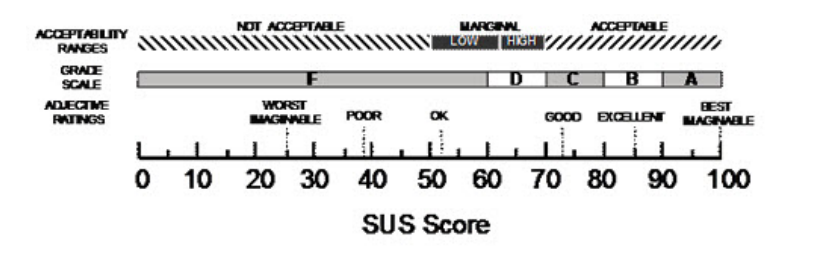
\includegraphics{pics/susscore}
		\caption{Nilai hasil evaluasi SUS}
		\centering
	\end{figure}
%-----------------------------------------------------------------------------%
\chapter{\babLima}
%-----------------------------------------------------------------------------%
Pada bab ini dibahas mengenai kesimpulan dari penelitian dan saran untuk penelitian
mendatang mengenai topik serupa.
%-----------------------------------------------------------------------------%
\section{Kesimpulan}
%-----------------------------------------------------------------------------%
Menjawab pertanyaan pertama pada rumusan masalah, dalam mengembangkan aplikasi video permainan harus mempertimbangkan beberapa hal. Pertama adalah jenis game yang akan dibuat, hal ini akan menjadi landasan dasar menentukan apa yang akan dilanjutkan selanjutnya. Kedua adalah menentukan elemen yang akan dibangun pada video permainan ini. Elemen tersebut adalah estetika, mekanik, naratif, dan teknologi. Dengan menentukan elemen ini maka semua syarat pembetukan sebuah game akan terpenuhi. Penentuan kedua hal tersebut akan didasari oleh pengguna dari aplikasi video permainan. Hal yang dibutuhkan untuk membentuk sebuah aplikasi video permainan untuk mata kuliah Dasar Dasar Pemrograman adalah sebuah rancangan sistem yang dapat memberikan nilai - nilai yang ada dalam tujuan mata kuliah Dasar Dasar Pemrograman. Memberikan sebuah materi tentang \textit{Computational Thinking} yang akan mengajarkan bagaimana sebuah logika komputer berjalan.
\linebreak\linebreak
Untuk menjawab pertanyaan kedua pada rumusan masalah, implementasi aplikasi video permainan untuk mata kuliah Dasar Dasar pemrograman mendapatkan respon yang cukup baik. Hasil kuantitatif untuk hasil evaluasi merupakan hasil dari UT yang dilakukan. Hasil dari UT adalah 78.57\% . Terdapat juga rekomendasi dari pengguna terkait aplikasi video permainan yang telah diterapkan. Hal tersebut akan terlihat jelas pada Subbab 4.6.

\section{Saran}
Saran yang akan diberikan merupakan pendapat dari penulis mengenai penelitian ini. Saran untuk penelitian ini adalah:
\begin{enumerate}
	\item Hasil penelitian ini diharapkan dapat berguna sebagai \textit{insight} untuk melakukan penelitan berikutnya, terutama penelitian yang terkait tentang pembelajaran menggunakan metode \textit{Game-Based Learning}
	\item Hasil \textit{Usability Testing} terutama bagian rekomendasi dapat menjadi dasar perbaikan apabila melakukan pengembangan aplikasi terkait maupun lanjutan.
	\item Mahasiswa dapat menemukan cara terbaik dalam mempelajari pemrograman karena telah mencoba metode ini.
	\item Peneliti lain dapat mengembangkan penelitian ini karena memiliki respon yang sangat baik dari mahasiswa Fakultas Ilmu Komputer.
	\item Materi pembelajaran \textit{Computational Thinking} dapat diajarkan sejak dini.
\end{enumerate}


%-----------------------------------------------------------------------------%
\chapter{\babEnam}
%-----------------------------------------------------------------------------%

%-----------------------------------------------------------------------------%
\section{Hasil Pengujian}
%-----------------------------------------------------------------------------%
%-----------------------------------------------------------------------------%
\subsection{Hasil Pengujian Kasus Uji 1}
%-----------------------------------------------------------------------------%
Tabel lain. Hasil tersebut dapat dilihat pada tabel \ref{tab:hasilgrrd}.
\begin{table}
	\centering
	\caption{Hasil pengujian menggunakan gromacs}
	\label{tab:hasilgrrd}
	\begin{tabular}{|c|l|*{3}{c|}}
		\rowcolor{headertbl}
  		\hline % create horizontal line
  		No & \f{Timestep} & \multicolumn{3}{|>{\columncolor{headertbl}}c|}{Waktu eksekusi berdasar jumlah prosesor} \\
		\hhline{|>{\arrayrulecolor{headertbl}}*{2}{-}>{\arrayrulecolor{black}}*{3}{|-|}}
  		\rowcolor{headertbl} & & 1 & 2 & 5 \\
  		\hline 1 & 200ps & 20h:27m:16s & 12h:59m:04s & 5h:07m:03s \\
  		\hline 2 & 400ps & 1d:22h:40m:03s & 1d:02h:08m:47s & 10h:09m:39s \\
  		\hline 3 & 600ps & 2d:23h:29m:21s & 1d:14h:52m:52s & 15h:25m:22s \\
  		\hline 4 & 800ps & 4d:02h:05m:57s & 2d:03h:30m:07s & 20h:29m:38s \\
  		\hline 5 & 1000ps & 5d:03h:29m:12s & 2d:16h:32m:22s & 1d:01h:34m:38s \\
  		\hline
	\end{tabular}
\end{table}
%-----------------------------------------------------------------------------%
\section{Evaluasi Hasil Kasus Uji}
%-----------------------------------------------------------------------------%
%-----------------------------------------------------------------------------%
\subsection{Evaluasi Kasus Uji 1}
%-----------------------------------------------------------------------------%
Tabel \ref{tab:hasilgrrd} menunjukkan hasil uji coba pada penelitian ini.  Gambar \ref{fig:grafgro5} menunjukkan perbandingan waktu eksekusi pada aplikasi x dengan jumlah prosesor sebanyak 5 buah.

\begin{figure}
	\centering
	\includegraphics[width=1\textwidth]
		{pics/5np-gromacs-chart.pdf}
	\caption{Perbandingan waktu eksekusi x untuk 5 prosesor}
	\label{fig:grafgro5}
\end{figure}
\paragraph{}
%-----------------------------------------------------------------------------%
\chapter{\babLima}
%-----------------------------------------------------------------------------%
Pada bab terakhir ini, 
%---------------------------------------------------------------
\section{Kesimpulan}
%---------------------------------------------------------------

%---------------------------------------------------------------
\section{Saran}
%---------------------------------------------------------------


%\printbibliography
%
% Daftar Pustaka
%\include{pustaka}
%biblama (bukan biblatex)
\bibliography{bib}{}
%\bibliography{references}{}
%biblama (bukan biblatex)
\bibliographystyle{apalikerd}
%\bibliographystyle{ieeetr} 

%
% Lampiran 
%
\begin{appendix}
	%
% @author  Andreas Febrian
% @version 1.00 
% 
% Hanya sebuah pembatas bertuliskan LAMPIRAN ditengah halaman. 
% 

\begin{titlepage}
	\centering 
	\vspace*{6cm}
	\noindent \Huge{LAMPIRAN}
	\addChapter{LAMPIRAN}
\end{titlepage}
	\setcounter{page}{2}
	%-----------------------------------------------------------------------------%
\addChapter{Lampiran 1 : Kuesoner \textit{Online}}
\chapter*{Lampiran 1 : Kuesoner \textit{Online}}
%-----------------------------------------------------------------------------%

%\begin{longtable}
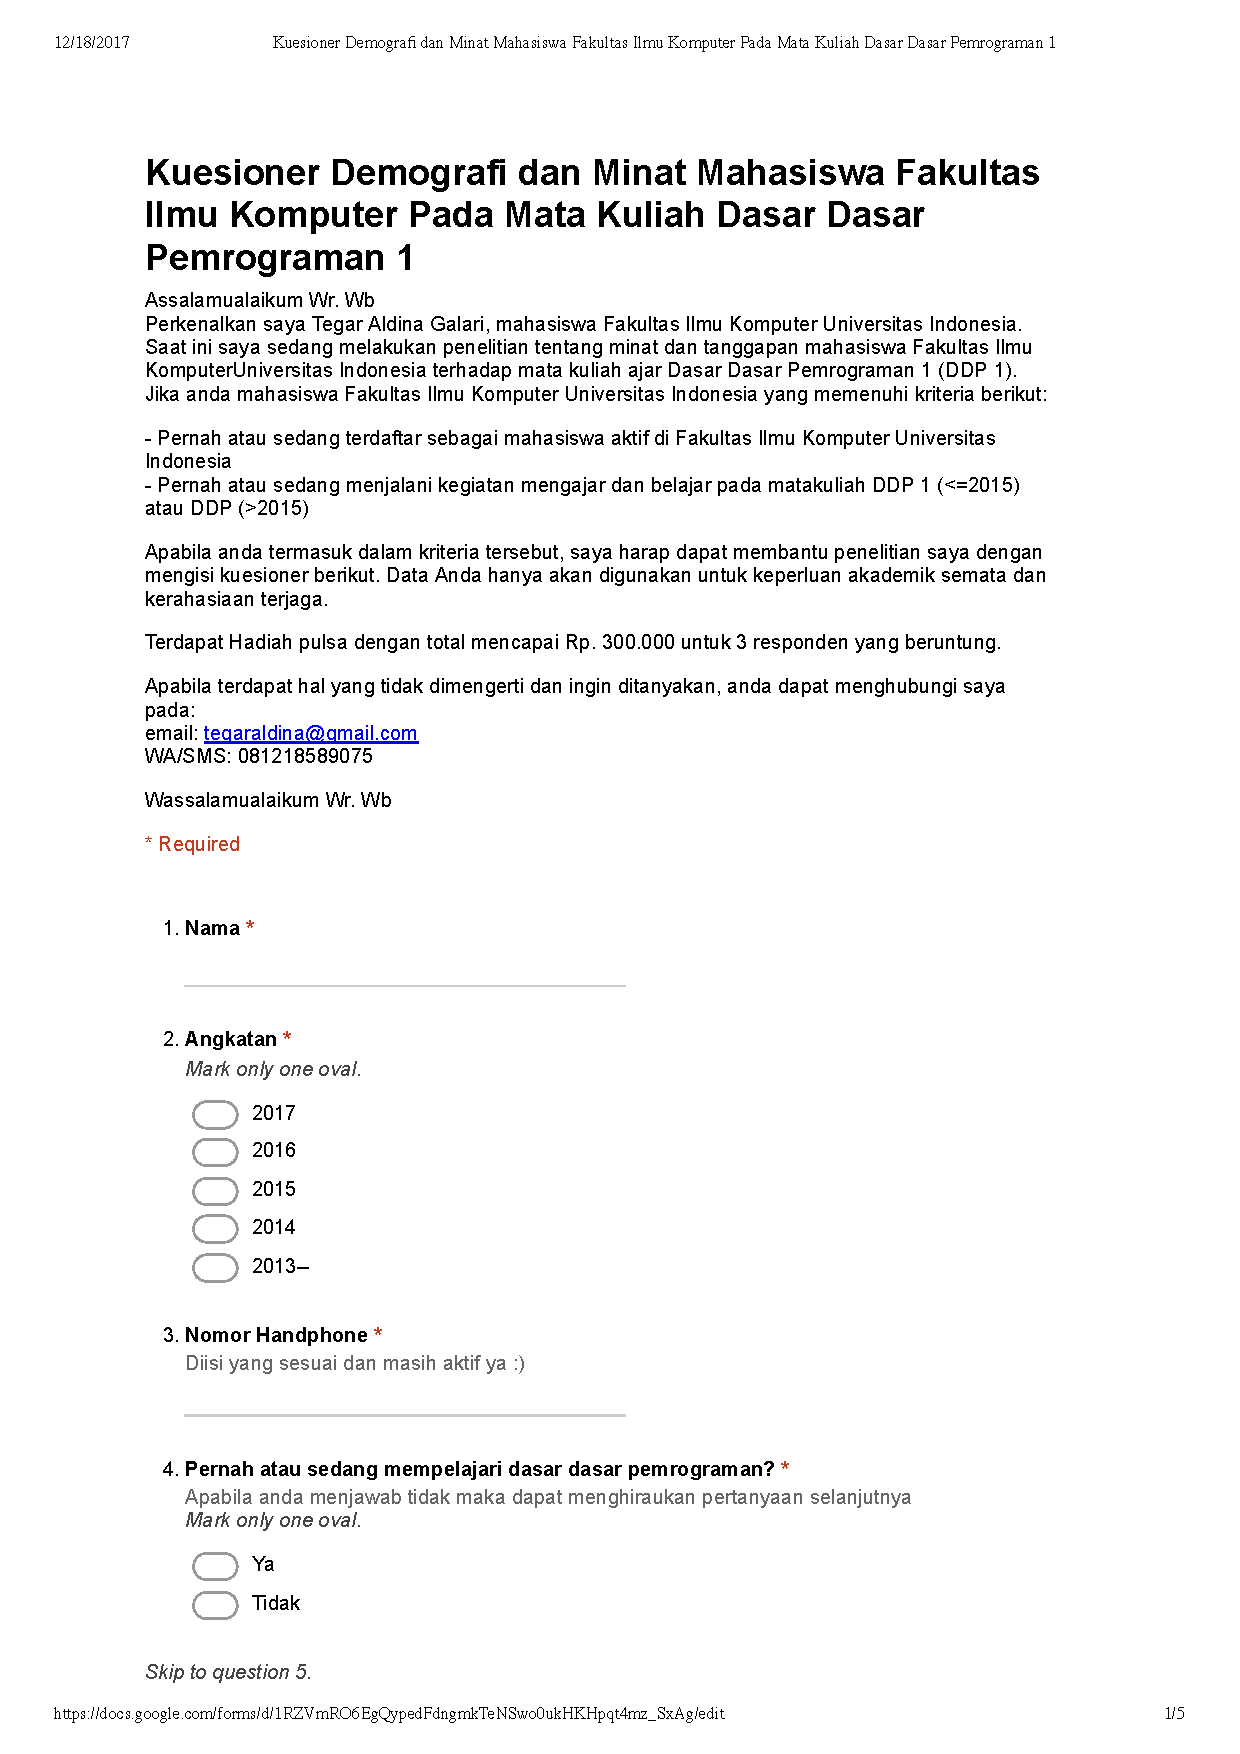
\includepdf[pages=-,pagecommand={},scale=0.6]{lampiran/Kuesoner-online.pdf}
%\end{longtable}

%-----------------------------------------------------------------------------%
\addChapter{Lampiran 2 : \textit{Form Usability Testing}}
\chapter*{Lampiran 2 : \textit{Form Usability Testing}}
%-----------------------------------------------------------------------------%
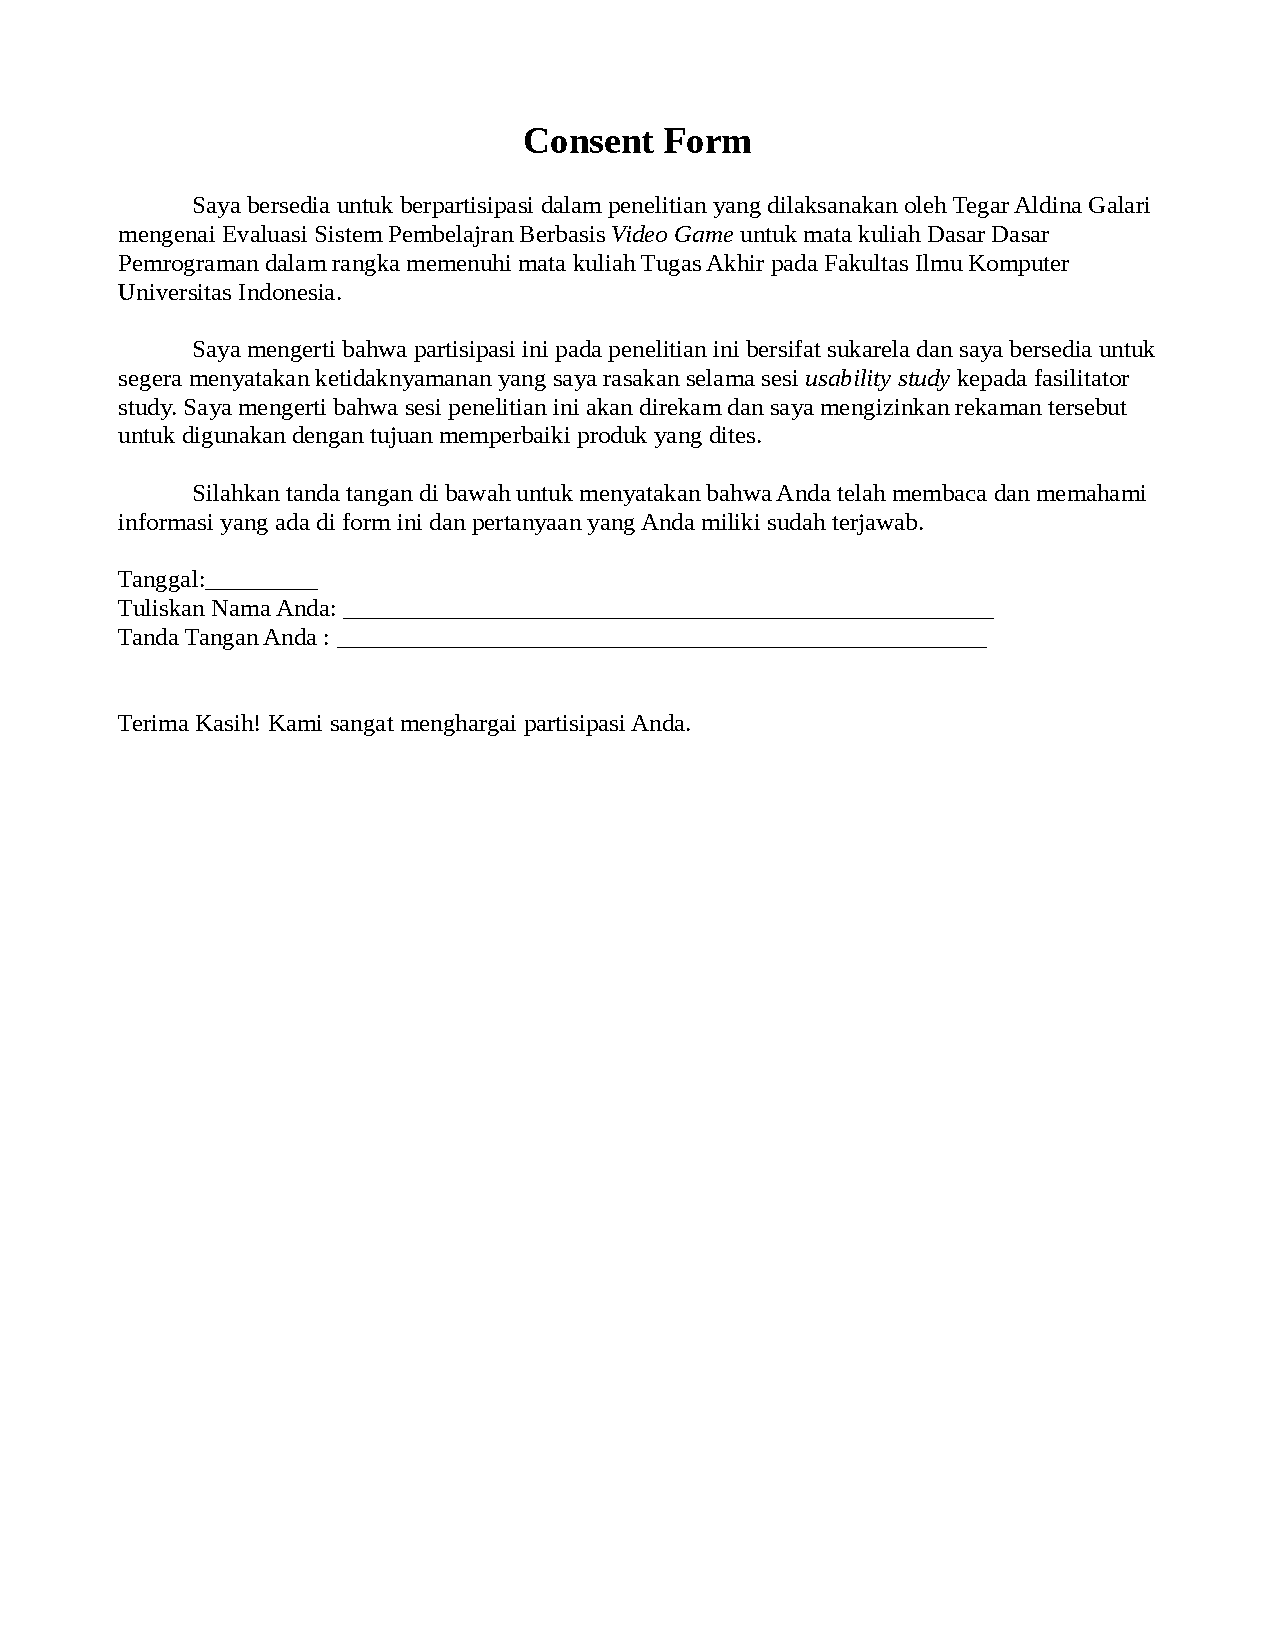
\includepdf[pages=-,pagecommand={},scale=0.9]{lampiran/form_UT.pdf}

\addChapter{Lampiran 3 : Hasil \textit{Usability Testing}}
%-----------------------------------------------------------------------------%
\begin{landscape}
	\chapter*{Lampiran 3 : Hasil \textit{Usability Testing}}
	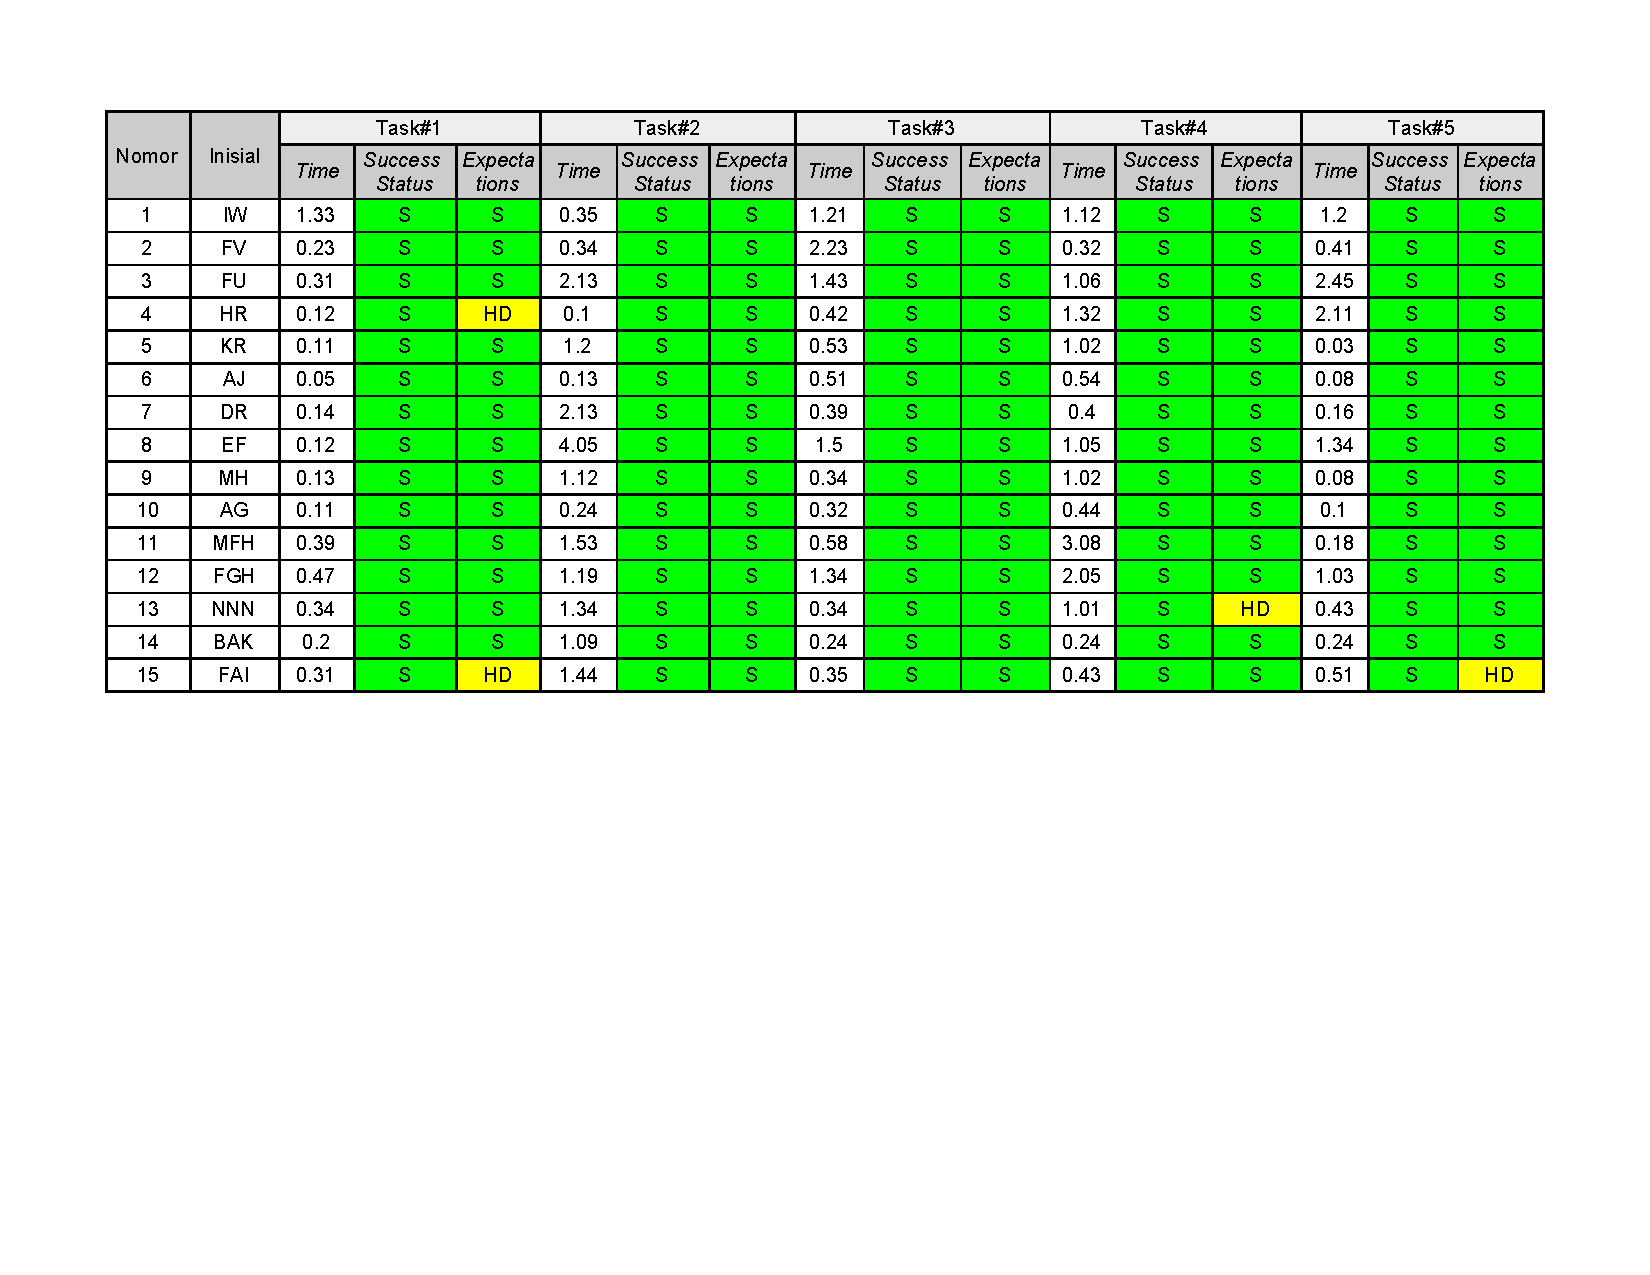
\includepdf[pages=-,pagecommand={},scale=1,angle=90]{lampiran/hasil-UT.pdf}
\end{landscape}

\end{appendix}

\end{document}